\documentclass[aspectratio=169,UTF-8]{ctexbeamer}

\usepackage{graphicx}
\usepackage{listings}
\lstset{language=C++,
                basicstyle=\ttfamily,
                keywordstyle=\color{blue}\ttfamily,
                stringstyle=\color{red}\ttfamily,
                commentstyle=\color{green}\ttfamily,
                morecomment=[l][\color{magenta}]{\#}
}

\usetheme{CambridgeUS}

\title{赫露艾斯塔\\ Helesta Compiler}
\author{焦景辉\ 王建楠\ 王子元\ 李欣隆}
\institute{清华大学}

\begin{document}

	\maketitle
	
	\begin{frame}
		\tableofcontents
	\end{frame}
	
	\section{整体架构}
	
		\begin{frame}{整体架构}
			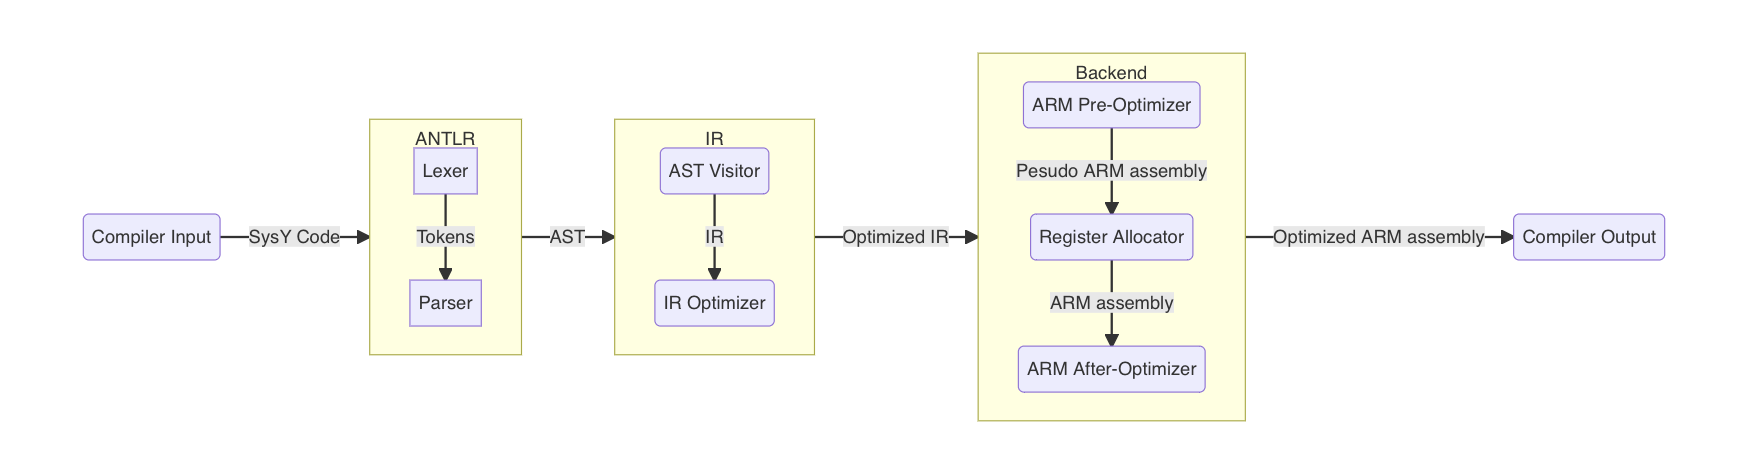
\includegraphics[width=\textwidth]{arch.png}
		\end{frame}
			
	\section{中端优化}
	
		\begin{frame}{SSA}
			\begin{itemize}
				\item SSA Construction: 构造 SSA,保证每个寄存器只有一次 Def
				\item SSA Destruction: 在中端优化的最后消除 $\Phi$ 指令
			\end{itemize}
		\end{frame}
		
		\begin{frame}{基本块优化}
			\begin{itemize}
				\item 消除不可达的基本块
				\item 消除分支条件可以推断为常量的分支
				\item 将基本块排列为正常顺序,使得同个循环内的代码是连续的若干个基本块,循环内的基本块按删去回边后 dfs 的逆后序排列
				\item 将无条件跳转的目标基本块的代码复制到跳转前的基本块,减少基本块个数
				\item 将基本块排列为正常顺序,使得同个循环内的代码是连续的若干个基本块,循环内的基本块按删去回边后dfs的逆后序排列
			\end{itemize}
		\end{frame}
		
		\begin{frame}{常规优化}
			\begin{itemize}
				\item Global Code Motion
				\item Global Value Numbering
				\item Dead Code Elimination: 消除无用指令 / 变量
				\item mem2reg: 全局变量转局部变量,局部变量放在寄存器上
			\end{itemize}
		\end{frame}
		
		\begin{frame}{过程间优化}
			\begin{itemize}
				\item Function Inline: 能 inline 的函数全部 inline,带递归的函数展开若干层
				\item 如果一个函数的某个参数在所有调用中相同,则将其替换为常量	
				\item 如果一个函数的返回值从未由调用者使用,则将返回值设为 0
				\item 尾递归转循环
				\item 用散列表保存单参数的递归函数的返回值
			\end{itemize}
		\end{frame}
		
		\begin{frame}{副作用优化}
			\begin{itemize}
				\item 对不写内存的函数调用,分析读的内存是否发生改变,消除多余的调用
				\item 对于数组没有被修改过的情况,将对数组的固定下标的访问替换为数组全局初始化的值
				\item 如果局部变量的每个下标都只被赋值过一次,且赋值为常数,则将其提升为全局常量
				\item 将 main 函数开头的全局变量写操作吸收到全局变量初始化中
				\item 尽可能将读内存操作替换为上次读或写的值
				\item 如果写操作不会对之后的读操作产生影响,则删除写操作
			\end{itemize}
		\end{frame}
		
		\begin{frame}{循环变换}
			\begin{itemize}
				\item 对于循环次数固定且展开后指令数较小的循环,展开为顺序执行
				\item 对于循环次数不固定的循环,进行循环展开
				\item 对于循环内部形如 \lstinline{s += i * c1 + c2}, \lstinline{s = (s + c1 * i + c2) \% P}, \lstinline{s /= 1 << c} 的表达式进行化简
			\end{itemize}
		\end{frame}
		
		\begin{frame}{代数化简}
			\begin{itemize}
				\item 加法表达式化简,将每个Reg表示为关于若干个Reg的线性函数,在能减少指令数时,直接计算这个线性函数而不是用原来的方式计算
				\item 如果 \lstinline{a / b} 已经计算过,那么将后续的 \lstinline{a \% b} 替换成 \lstinline{a - a / b * b}
				\item 将 \lstinline{a * b / b} 替换成 \lstinline{a}
			\end{itemize}
		\end{frame}
		
		\begin{frame}{SIMD 与多线程}
			手动实现一个多线程库
			
			\begin{itemize}
				\item \lstinline{__create_threads}:利用系统调用 \lstinline{sys_clone} 创建线程
				\item \lstinline{__join_threads}:利用系统调用 \lstinline{sys_exit} 和\lstinline{sys_waitid} 结束线程或等待线程结束
				\item \lstinline{__bind_core}:利用系统调用将线程绑定到 CPU 核心
				\item \lstinline{__lock}:互斥锁进入操作,用于修改已结束的线程数
				\item \lstinline{__unlock}:互斥锁退出操作,用于修改已结束的线程数
				\item \lstinline{__barrier}:barrier,用于线程间同步
			\end{itemize}
			
		\end{frame}
		
		\begin{frame}{SIMD 与多线程}
			\begin{itemize}
				\item 多线程:对于一个 $k$ 次迭代的循环,如果判断循环间无数据依赖,则将其分为 $\frac{k}{\mathrm{num\_threads}}$ 块并行执行
				\item SIMD:如果一个循环中没有分支,且每次循环间无数据依赖,且每条指令都能换成 SIMD 指令,且 SIMD 寄存器够用,则替换为 SIMD 指令
			\end{itemize}

		\end{frame}
	
	\section{后端优化}
	
		\begin{frame}{常规优化}
			\begin{itemize}
				\item Dead Code Elimination
				\item 对只含一条跳转指令的基本块,尽可能删除,但保证不出现基本块间的多重边
				\item 对只有一个前驱的基本块,将指令移动到前驱
				\item 分支指令转为条件执行
			\end{itemize}
		\end{frame}
		
		\begin{frame}{指令合并}
		
			\begin{itemize}
				\item 将 \lstinline{a + b * c} 和 \lstinline{a - b * c} 替换成 \lstinline{mla} 和 \lstinline{mls}
				\item 将多条 \lstinline{store} 替换成 \lstinline{vdup} 和 \lstinline{vstm}
				\item 如果多条 \lstinline{load / store} 地址相差不超过 1024,则只计算第一次地址,后续地址使用偏移量
				\item 将形如 \lstinline{a[b]} 的数组访问使用 \lstinline{(ldr|str) a,[b,c,LSL 2]} 表示
			\end{itemize}
		\end{frame}
		
		\begin{frame}{寄存器分配}
			\begin{itemize}
				\item 基于图染色问题的寄存器分配算法,优先保证生成代码的运行速度。
				\item 对 \lstinline{int} 和 \lstinline{float} 类型的伪寄存器分别执行寄存器分配。
				\item spill估价:优先spill保存常量的寄存器,优先spill使用频率较低的寄存器。
				spill策略考虑伪寄存器所在的循环深度\lstinline{depth} 与使用次数 \lstinline{cnt},计算$cnt * 4^{depth}$。
				\end{itemize}
		\end{frame}
	
\end{document}